\documentclass[oneside, 12pt, a4paper]{book}

% Aufgaben 
\usepackage{todonotes}
% Seitenlayout 
\usepackage[ % Seitenlayout bestimmen für das gesamte Dokument
	left=2.5cm,
	right=3.5cm,
	top=2.5cm,
	bottom=2cm,
	%includeheadfoot
]{geometry}
\usepackage[T1]{fontenc} % Westeuropäische Sprachen werden hiermit unterstützt
\usepackage[ngerman]{babel}
\usepackage{times} % Times New Roman Schriftart 
\usepackage[onehalfspacing]{setspace} % 1.5 Zeilenabstand
\usepackage{acronym} % Abkürzungen & Abkürzungsverzeichnis
\usepackage{graphicx} % Bilder einfügen in das Dokument
\usepackage[hidelinks]{hyperref} % Kreuzreferenzen & Verlinkung


% Quellen:
\usepackage[backend=biber, style=authoryear]{biblatex} %BibLaTeX zum zitieren
\usepackage[autostyle=true]{csquotes}
\addbibresource{sources.bib}

% Import of the different Shortcuts
%%%%%%%%%%%%%%%%%%%%%%%%%%%%%%
% Shortcuts for the Document %
%%%%%%%%%%%%%%%%%%%%%%%%%%%%%%

% Arbeit
\newcommand{\titleDoc}{Generische Gestaltung von Projekten im Bereich Customizing von Standardsoftware.}
\newcommand{\wissenschaftlicheFrage}{\emph{Wie kann ein Projekt im Bereich des Customizings von Standardsoftware generisch gestaltet werden? }}

% Hochschule
\newcommand{\prueferA}{Prof. Stefan Stock}
\newcommand{\institution}{EUFH Brühl}
\newcommand{\institutionAdress}{Kaiserstraße 6 \\50321 Brühl}
\newcommand{\autorStudiengang}{Digitales Projektmanagement}

% Autor
\newcommand{\autor}{Jakub Rzasa}
\newcommand{\autorMatrikelnummer}{21961012}
\newcommand{\autorStrasse}{Hindenburgstr. 5}
\newcommand{\autorPLZ}{51103}
\newcommand{\autorOrt}{Köln}
\newcommand{\autorGeburtsort}{Konstanz}
\newcommand{\autorGeburtsdatum}{21.04.1995}





\begin{document}
	
	% Vorderer Abspann
	\frontmatter
	
	\pagenumbering{Roman}
	\thispagestyle{plain}

\begin{titlepage}
	\centering
	
\includegraphics[width=0.5\textwidth]{img/EUFHTitle.png}\par\vspace{1cm}
	{\scshape\LARGE \institution\par}
	\vspace{1cm}
	{\scshape\Large \autorStudiengang\par}
	\vspace{1.5cm}
	{\huge\bfseries \titleDoc\par}
	\vspace{2cm}
	{\Large\itshape \autor\par}
	\vfill
	Betreuer: \par
	\textsc{\prueferA}
	
	\vfill
	
	% Bottom of the page
	{\large \today\par}
\end{titlepage}


	
	
	\thispagestyle{plain}
\chapter{Abstract}
\label{sec:einleitung}

	
	Der Projekterfolg hängt heutzutage maßgeblich von der Termintreue , der Budgettreue sowie dem Endergebnis ab. Wird einer dieser Faktoren vernachlässigt, so kann ein Projekt sich verzögern oder sogar abgebrochen werden. Dies hat nicht nur eine negative Auswirkung auf das Unternehmen, welches das Projekt durchgeführt hat, sondern verschlingt auch Unmengen an Ressourcen die anderweitig eingesetzt werden können. Um dieses Geschehnis vorzubeugen, entstanden in den vergangenen Dekaden einige Ansätze des Projektmanagements. Jeder Ansatz verfügt über seine eigenen Werkzeuge die einem Projektmanager dabei helfen ein Projekt zum richtigen Zeitpunkt, mit dem richtigen Budget, sowie der richtigen Qualität abzuschließen. Im Bereich des Custoimzings, in dem Kunden sich darauf verlassen, das die Anpassung so effizient wie möglich erstellt wird, sodass mit dem System fehlerfrei gearbeitet werden kann, ist eine genaue Terminierung, sowie eine damit einhergehende Transparenz wichtig. 

	Die gicom AD ist ein SAP Beratungshaus mit Hauptsitz in Overath. Die mittlerweile mehr als 70 Beschäftigten beraten Kunden rund um das Thema Verhandlungsplanung, Verhandlungsvorbereitung, Verhandlungsstrategieentwicklung, sowie der Abrechnung. Bei der von der gicom zur Verfügung gestellten Software handelt es sich um eine Standardsoftware, welche zusammen mit dem Kunden angepasst wird. Die Software teilt sich in drei unterschiedliche Module von denen sich eines mit der Digitalisierung, das zweite mit der Berechnung unterschiedlicher Ansprüche, sowie das dritte mit der Verhandlung selbst beschäftigt. Jedes dieser Module benötigt eine separate Anpassung an die Unternehmensumgebung des Kunden. Ziel dieser Arbeit ist es ein Strukturiertes vorgehen im Customizing zu erkennen, anhand dessen ein generisches Modell entstehen kann welches dem Benutzer eine Handlungsempfehlung an die Hand gibt. Dadurch soll die Aufgaben Findung  erleichtert sowie eine Stringenz bei der Notation geschaffen werden.
	
	Die Wissenschaftliche Frage, die sich aus dem Titel der Arbeit ableitet, lautet:
	
	\begin{quote}
		\wissenschaftlicheFrage
	\end{quote}

	Für eine strukturierte Bearbeitung der Wissenschaftlichen Frage wurden drei Unterfragen gebildet, anhand derer die Ausarbeitung gegliedert wird. 
	
	\begin{enumerate}
		\item \ersteUnterfrage
		\item \zweireUnterfrage
		\item \dritteUnterfrage
	\end{enumerate}

	Die Fragen werden der Reihenfolge entsprechend abgearbeitet. Im \autoref{chap:projektablauf} wird somit geklärt, wie ein Projekt aussieht. Das \autoref{chap:SpecCustom} befasst sich mit den einzelnen Phasen eines Projektes. Hier werden die verschiedenen Ansätze des Projektmanagement erläutert. Während im \autoref{chap:umsetzung} ein Modell, zur allgemeinen Lösung eines solchen Problems, erstellt wird, befasst sich das \autoref{chap:handlungs} mit der Anwendung dieses Models auf die gicom AG. 
	

	

	\tableofcontents
	\listoffigures
	\chapter{Abkürzungsverzeichnis}

% Change lengths for nicer output
\newlength{\olditemsep}
\newlength{\oldparskip}
\setlength{\olditemsep}{\itemsep}
\setlength{\oldparskip}{\parskip}
\setlength{\itemsep}{2pt}
\setlength{\parskip}{2pt}

\begin{acronym}[title=Abkürzungsverzeichnis]
	\acro{LZ}{Lebenszyklus}
	\acro{PSP}{Projektstrukturplan}
	\acro{AP}{Arbeitspaket}
	\acro{UI}{User Interface}
	\acro{AD}{Agreement Documentation}
	\acro{RTM}{Real-Time-Margin}
	\acro{ANW}{Agreement Negotiation Workbench}
	
\end{acronym}

% Reset lengths
\setlength{\itemsep}{\olditemsep}
\setlength{\parskip}{\oldparskip}


% mit \acp{abkürzung} kann ich Abkürzungen refferieren
	\newpage
	
	
	% Hauptdokument
	\mainmatter
	\chapter{Projektplanung}
\label{chap:projektablauf}

	In diesem Kapitel wird der Begriff Projekt abgegrenzt, sowie auf die unterschiedlichen Projektphasen eingegangen. Diesbezüglich dient dieses Kapitel zur Klärung der Frage: \ersteUnterfrage

\section{Projekt}

	Die Ursache für die Entstehung eines Projektes, liegt primär in einem ungedeckter Bedarf. Für die Erfüllung eines solchen Bedarfs fallen mehrere unterschiedliche Aufgaben, die von Menschen aus unterschiedlichen Bereichen, Abteilungen, Unternehmen oder in einigen Fällen Ländern erfüllt werden, an. Jeder dieser Mitarbeiter ist ein essentieller Bestandteil des Projektfortschritts. Die zu erfüllenden Aufgaben werden Kategorisiert, sowie in einen Zeitlichen Zusammenhand gesetzt.\cite[4]{Wysocki_2019_Projekt}
	
	Diese aneinander gereihten Aufgaben werden Teilprozesse genannt und tragen entscheidend zu der Fertigstellung eines größeren Vorhabens, welches Prozess genannt wird, bei. Madauss beschreibt ein Projekt als \enquote{\textit{Vorhaben mit definiertem Anfang und Abschluss, das durch die Merkmale zeitlicher Befristung, Einmaligkeit, Komplexität und Neuartigkeit gekennzeichnet ist.}}\cite[4]{Madauss2020} Die ISO Norm bezeichnet diese Art von Vorhaben als eine \enquote{Gruppe von Prozessen}\cite[11]{ISO10006_2019}, welche zusammen ein ganzes ergeben. Somit ist ein Projekt durch die folgenden Punkte gekennzeichnet: 
	
	\begin{itemize}
		\item Einzigartigkeit 
		\item Komplexität
		\item Zusammenhängende Aktivitäten
		\item Bestehend aus mehreren Teilprozessen
		\item Zeitliche Befristung 
		\item Einem gemeinsamen Ziel
		\item Einem bestimmten Budget
	\end{itemize}
	
	Unter der Berücksichtigung der oben erwähnten Punkte, lässt sich ein Projekt also als ein einmaliges Vorhaben beschreiben, welches ein bestimmtes Ziel verfolgt, eine gewisse Komplexität mit sich bringt und über ein vorgegebenes Budget verfügt. \cite[4-7]{Wysocki_2019_Projekt}
	Die Erreichung wird durch Projektphasen gewährleistet, die neben der Überwachung des Fortschritts auch die noch zu erreichenden Teilziele abdecken. 
	
\section{Lebenszyklus}
	
	Projekte können Abhängig von der Größe, sowie der Branche in welcher sie durchgeführt werden, mehrere Wochen oder Jahre dauern. So kann sich Beispielsweise die Entwicklung einer Software über mehrere Jahrzehnte ziehen. Die Bearbeitung eines solchen Vorhabens unterteilt sich grundsätzlich in logisch aufeinander folgende Phasen, die das Projektmanagements von der Definition der Zielvorgabe bis zum Abschluss begleiten. Sie stellen außerdem das Grundkonzept des Projektmanagements dar.\autocite[107-110]{madauss2019} Jede Phase steht hierbei für einen in sich geschlossenen Teil des Projektes, der über die Definition der Hauptaufgabe in der jeweiligen Phase verfügt, sowie eine Auskunft über das genaue vorgehen in der Phase gibt. Eine Phase beschreibt außerdem durch die Definition von Meilensteinen genau welche Aufgaben nach Abschluss einer Phase erledigt sein müssen. Bei der Abnahme dieser Phase dienen die Meilensteine als Abnahmekriterien anhand dessen der Fortschritt festgestellt werden kann.\autocite[16]{Meyer2020}
	
	Zusammengefasst werden diese Phasen unter dem Begriff \ac{LZ} eines Projektes verstanden. Ziel des Lebenszyklus ist es, ein klares Vorgehen im Projekt zu schaffen, wodurch ein nachvollziehbarer Projektplan entstehen kann und somit auch eine Baseline. Als baseline bezeichnet man einen Projektplan, der den Grundstein eines Projektes darstellt. Je nach Branche kann sich der \acs{LZ} eines Projektes unterscheiden.\autocite[14]{Meyer2020} In der IT-Branche beispielsweise gibt es auch Branchenintern einige geringfügige Unterschiede. So spricht die ISO-Norm von fünf Projektphasen \autocite[11]{DIN69901-2}, während das amerikanische Project Management Institute lediglich von vier Phasen spricht. Die PRINCE2 geht einen schritt weiter und definiert lediglich zwischen zwei Abschnitten, nämlich des Initiierung und dem Ende. Es lässt gewollt Spielraum für die mittleren Phasen übrig, da die sich je nach zu erbringender Leistung unterscheiden\autocite[15]{Meyer2020}. Die Abbildung \ref{img:phasen} veranschaulicht die unterschiedlichen Herangehensweisen der definierten Standards. 
	
	\begin{figure}[h]
		\centering
		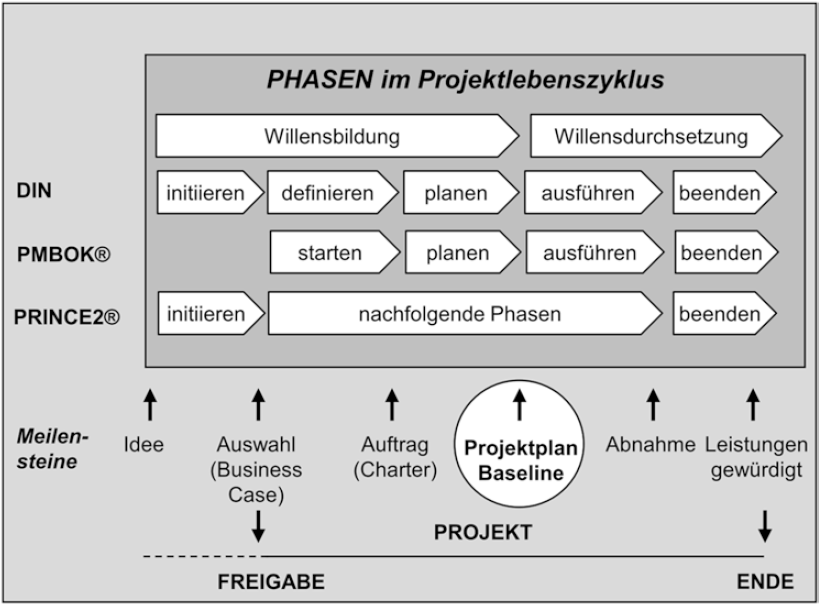
\includegraphics[width=15cm]{img/Projektlebenszyklus.png}
		\caption{Phasen der unterschiedlichen Normen\cite[15]{Meyer2020}}
		\label{img:phasen}
	\end{figure}

	Jede einzelne Phase übernimmt somit einen eigenen Bereich eines Projektes. Die Bereiche einer jeden Phase hängen von den Ergebnissen der vorherigen Phase ab\autocite[16]{Meyer2020}. Im folgenden werden die Phasen beschrieben: 
	
	\begin{enumerate}
		\item Initiierungsphase	
			\subitem Am Ende dieser Phase wird entschieden ob eine Projektidee zu einem realen Projekt wir, oder ob sie verworfen wird. Dies kann durch unterschiedliche Analysen untersucht werden, die jedoch nicht Teil dieser Arbeit sind.
			
		\item Definitionsphase
			\subitem In dieser Phase wird die Idee Konkretisiert, sowie geplant. Somit müssen die unterschiedlichen Stakeholder eingeweiht werden. Die Projektleitung muss aufgestellt werden. 
		\item Planungsphase
			\subitem In der Planungsphase erstellt das Projektteam bzw. der Projektleiter Pläne für die Durchführung des Vorhabens. Die primär berücksichtigten Faktoren bei der Planung sind Kosten, Qualität und Zeit. Der Projektleiter erstellt einen Projektstrukturplan, der das weitere Vorgehen eines Projektes bestimmen soll. 
		\item Umsetzphase
			\subitem In dieser Phase wird die hauptsächliche Leistung erbracht. Der Projektmanager ist hier primär mit der Überwachung und Steuerung des Projektes beschäftigt. 
		\item Abschlussphase
			\subitem Mit dieser Phase wird der Abschluss eines Projektes eingeläutet. Hier wird sowohl die erzielte Leistung als auch die Dokumentationen übergeben. Des weiteren werden Lessons-Learned aus dem Projekt gezogen sowie die Ressourcen zurück zu deren ursprünglichen Aufgaben zurückgeführt. 
						
	\end{enumerate}

	Diese Aufteilung eines Projektes in einzelne Projektphasen, gewährleistet nicht nur mehr  Kontrolle über die einzelnen Aktivitäten im Projekt, sondern ermöglicht es auch eine genauere Planung im Projekt durchzuführen. Durch eben diese Kontrolle können die Qualität, Kosten, Termine sowie Leistungsergebnisse im falle einer Abweichung frühzeitig identifiziert sowie korrigiert werden.\cite[57]{Känel_2020_Projektphasen}
	
	
\section{Projektphasenmodelle}
\label{sec:phasenmodell}

	Ein Phasenmodell wird folgendermaßen Definiert:
	
	\begin{quote}
		\enquote{\textit{Unter einem \textbf{Phasenmodell} ist im Rahmen des Projektmanagements eine weitgehend
		standardisierte Darstellung der Gliederung eines typischen Projektablaufs
		in sachliche und zeitliche Abschnitte zu verstehen.
		Diese Abschnitte müssen sich eindeutig bezeichnen lassen und dienen vor allem
		der Orientierung und Standortbestimmung im jeweiligen Projektablauf.}}\autocite[57]{Känel_2020_Projektphasen}
	\end{quote}
	
	Laut Känel stellen Phasenmodelle somit einen Rahmen dar, der einen Projektmanager bei der Planung und Kontrolle unterstützt. Die zu der Orientierung dienenden Rahmenwerke gibt es in unterschiedlichen Ausprägungen. Bei der Betrachtung solcher Modelle im Zusammenhang mit digitalem Projektmanagement lassen sich Grundsätzlich drei Ansätze unterscheiden. Das klassische Vorgehen im Projektmanagement, bei diesem Ansatz wird davon ausgegangen, dass ein Projekt von dem \enquote{Anfang} bis zum \enquote{Abschluss} durchgeplant werden kann. Somit werden die einzelnen Phasen möglichst genau vorausgeplant. Wodurch die einzelnen Phasen nach dem Plan sequentiell abgearbeitet. Ein typisches Vorgehensmodell für diesen Ansatz ist das \enquote{Wasserfallmodell} oder auch das \enquote{V-Modell}\autocite[Kap. 2]{Vivenzio2013}. Die Abbildung \ref{img:wasserfall} zeigt die typischen Phasen des Wasserfallmodells 

	\begin{figure}
		\begin{minipage}[b]{.4\linewidth} % [b] => Ausrichtung an \caption
			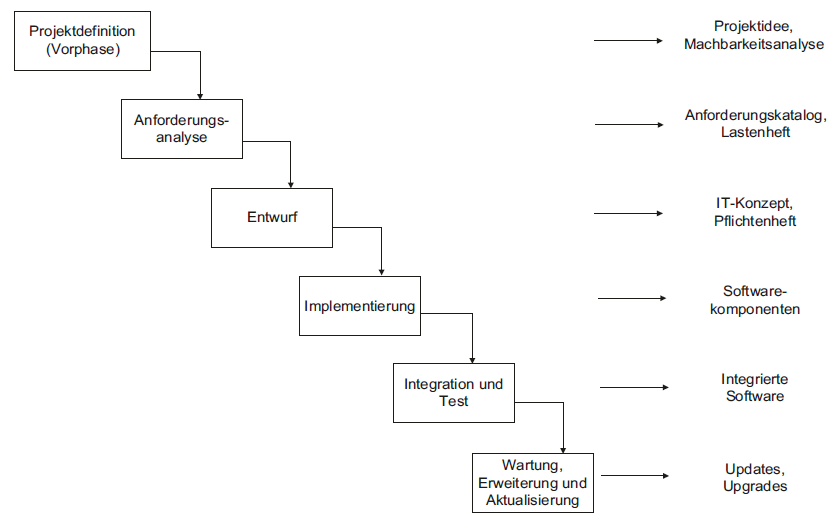
\includegraphics[width=8cm]{img/wasserfallmodell.png}
			\caption{klassisches Vorgehen: Wasserfallmodell \autocite[353]{Alpar2019}}
			\label{img:wasserfall}
		\end{minipage}
		\hspace{.1\linewidth}% Abstand zwischen Bilder
		\begin{minipage}[b]{.4\linewidth} % [b] => Ausrichtung an \caption
			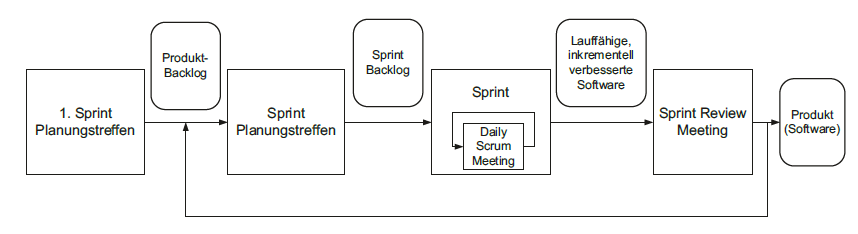
\includegraphics[width=8cm]{img/scrum.png}
			\caption{agiles Vorgehen: Scrum \autocite[372]{Alpar2019}}
			\label{img:scrum}
		\end{minipage}
	\end{figure}
	
	Der ein weiterer Ansatz des Projektmanagements ist das agile Vorgehen. Bei dem primär in der Softwareentwicklung genutzten Ansatz liegt das Augenmerk auf der Agilität, die durch das verbesserte eingehen auf den Kunden gewährleistet wird. Dadurch werden die einzelnen Phasen nicht genau durchgeplant, vielmehr wird eine iterative Vorgehensweise angestrebt, bei welcher der Kunde stets berücksichtigt wird. Ein Typisches Modell dafür ist \enquote{SCRUM}. Dieses Modell wird anhand von fest definierten Zeitabschnitten, welche \enquote{Sprints} genannt werden, abgearbeitet.\autocite[57-70]{Känel_2020_Projektphasen}\autocite[Kap. 1.3]{Alam2020}
	Die Abbildung \ref{img:scrum} beschreibt den Prozess der agilen Vorgehensweise Scrum.
	
	Bei der Umsetzung von Projekten in der Praxis ist eine solche saubere Abgrenzung zwischen der klassischen, sowie der agilen Vorgehensweise oft nicht möglich, daher gewinnen Kombinationen der beiden ersten Ansätze an Bedeutung. Diese hybriden Vorgehensweisen entnehmen einzelne Phasen oder Teilprojekte aus den entsprechenden Konzepten und kombinieren sie mit einem anderen  Ansatz. 
	So kann es beispielsweise sein, dass ein Softwareentwicklungsprojekt die Phasen der Projektdefinition, Anforderungsanalyse und Entwurf aus dem Wasserfallmodell entnehmen, die Implementierung und Integration jedoch agil gestaltet wird.\autocite[65]{Känel_2020_Projektphasen}
	
	Die genannten Ansätze unterscheiden sich zwar von der Vorgehensweise, zielen jedoch alle auf eine Strukturierung von Projekten ab, wodurch eine Wertsteigerung gewährleistet werden kann. Ein zentrales Werkzeug für die Sicherstellung der Qualität bei der Planung in Projekten ist der Projektstrukturplan. Durch ihn können den Phasen einzelne Arbeitspakete zugeordnet werden, die es abzuarbeiten gilt. 

\section{Projektstrukturplan}
	Der \ac{PSP} ist laut der DIN 69901-5 Norm eine \enquote{vollständige hierarchische
	Darstellung aller Elemente (Teilprojekte, Arbeitspakete) der Projektstruktur als
	Diagramm oder Liste}\autocite{DIN_Projektplan}
	Er fasst die unterschiedlichen Phasen zusammen und ordnet ihnen Aufgaben zu. Somit kann nicht nur der Fortschritt besser gemessen, sondern auch die Zuordnung der Verantwortlichkeiten im Projekt zugeteilt werden. 
	
	Aufgebaut wird der \acs{PSP} hierarchisch, die Hierarchie wird nach einem Top-Down bestimmt. Im Folgenden die hierarchische Gliederung des \acs{PSP}: 
	
	\begin{enumerate}
		\item \textbf{Projekt}
			\subitem Hier werden im \acs{PSP} sowohl die Ziele des gesamten Projektes dokumentiert als auch der Projektauftrag. 
			
		\item \textbf{Teilprojekte/ Projektphasen}
			\subitem Diese Phasen dienen der allgemeinen Übersicht über den Projektablauf. Jede Phase besitzt meistens einen Teilprojektleiter, der für die Fertigstellung seines Teils verantwortlich ist. 
		
		\item \textbf{Arbeitspakete}
			\subitem Arbeitspakete sorgen für eine klare Struktur der Aufgaben. Sie fassen eine bestimmte Zahl von Aufgaben zu einem Paket zusammen. Das Ziel ist eine eindeutige Zuordnung von Kosten, Ressourcen und Zeitaufwand zu schaffen. Die Namensgebung muss daher eindeutig gewählt werden, damit eine Abgrenzung möglich ist. Ein Arbeitspaket umfasst den Namen des verantwortlichen Bearbeiters, die Aufgabenbeschreibung, Abnahmebedingungen, den Bearbeitungsaufwand sowie den Ressourcenbedarf. 
		
		\item \textbf{Aufgaben}
			\subitem Sind die kleinste Einheit in einem Projekt. Sie beschreiben die zu erbringende Tätigkeit in dem Arbeitspaket. 
		
	\end{enumerate}

	Neben der hierarchischen Aufteilung besitzt der \ac{PSP} mehrere Möglichkeiten einer Gliederung. 
	
	\begin{itemize}
		\item Verrichtungsorientiert
			\subitem Aufgaben die erfüllt sein müssen, damit das Projekt verwirklicht wird.
		
		\item Objektorientierung
			\subitem Plant Ergebnisse sowie Lieferobjekte die im Laufe der Phase/ Projektes zu erledigen sind. 
		
		\item Phasenorientierung
			\subitem Orientiert sich an den Phasen aus dem Projektmanagement
	\end{itemize} 

	Wegen der Komplexität heutiger Projekte, sowie deren mehrdimensionaler Projektstruktur kommt es nicht selten zu einer Mischform dieser Gliederungsarten. \autocite[387-391]{Alpar2019}

\section{Arbeitspakete}
\label{sec:arbeitspakete}

	Unter einem \ac{AP} wird die Beschreibung der Aufgabe im Prozess bezeichnet, die von einer Person bzw. einer Abteilung in der festgelegten Zeit zu mit dem vereinbarten Aufwand zu vollbringen ist.\autocite[196]{Känel_2020_Projektphasen} In einem Arbeitspaket werden daher unterschiedliche Informationen festgehalten, die einem Projektmanager helfen eine Planung durchzuführen. Es wird neben der Beschreibung auch eine eindeutige Nummer, die Start und Ende Zeit, die Kosten, der Ressourcenbedarf etc. festgelegt. Die \autoref{img:arbeitspaket} zeigt ein beispielhaftes Layout. 
	
	\begin{figure}[h]
		\centering
		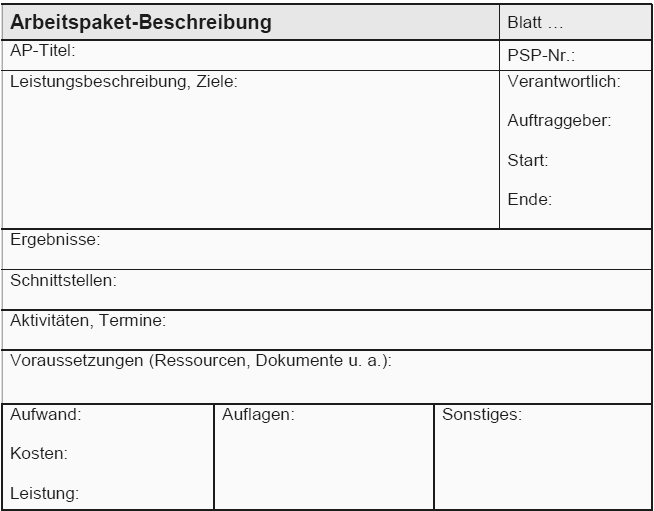
\includegraphics[width=15cm]{img/Arbeitspacket.png}
		\caption{Phasen der unterschiedlichen Normen\autocite[170]{Känel_2020_Projektphasen}}
		\label{img:arbeitspaket}
	\end{figure}
	
	
	
	
	
	
	
	
	
	
	
	
	
	\chapter{Spezifika von Customizing Projekten}
\label{chap:SpecCustom}

	Dieses Kapitel befasst sich mit der Fragestellung \dritteUnterfrage Hier soll ein Einblick in die Aufgaben eines Consultants gegeben werden, sowie herausgearbeitet werden, welche Aufgaben zu erledigen sind.  
	
\section{Customizing}

	Das Customizing befasst sich laut dem Gabler Wirtschaftslexikon mit der \enquote{Anpassung von Standardsoftware an kundenindividuelle Anforderungen.}\autocite{Lackes_customizing}
	Das Ziel ist es, eine programmierte Software mit kundenindividuellen Daten zu befüllen. Da es sich bei der gelieferten Standardsoftware, im Gegensatz zu einer Individualsoftware, um eine nicht an die Kundenumgebung angepasste Software, welche an unterschiedliche Kunden angepasst werden kann, handelt, muss eine Anpassung vorgenommen werden. 
	Das Customizing einer Software verlangt auf der einen Seite die Anpassung der Software selbst. Indem unterschiedliche Module ausgewählt werden können, kann ein Kunde die von ihm benötigten auswählen, wodurch nur die in Rechnung gestellt werden, die wirklich genutzt werden. Auf der anderen Seite müssen die Daten in der Software angepasst werden. Hierbei handelt es sich um Schnittstellen, Spracheinstellungen, sowie \ac{UI} Einstellungen. Abschließend müssen Daten an das an den Kunden angepasste System eingespielt werden. Dies passiert entweder durch die Nutzung des neuen Systems oder durch Migration von Daten aus dem alten auf das neue System. \autocite[668-669]{Hansen2009} 
	
\section{SAP Customizing}
\label{sec:sapCustomizing}
	
	Für eine ordnungsgemäße Nutzung der SAP Software muss stets ein Customizing vorgenommen werden. Im Rahmen der Transformation der von den R/3 auf die S/4 HANA Systeme hat die SAP einen eigenen Ansatz des Customizing herausgebracht. Der unter dem Namen SAP Activate laufende Ansatz umfasst sechs Phasen, sowie einen Iterations-Kreis der Phasen unabhängig ist. Die benennung fand eir folgt statt: Discover, Prepare, Explore, Realize, Deploy, sowie Run\autocite[331]{Denecken2020}

\section{Aufgaben im Customizing}
	\label{sec:aufgabenCustomizing}
	
	Für derartige Anpassungen der Standardsoftware fallen die folgenden Arten von Aufgaben an: 
	
	\begin{itemize}
		\item Modulauswahl
			\subitem Auswählen ist eine zentrale Aufgabe im Customizing, da nicht immer klar ist welche Module der Kunde benötigt. Daher müssen anhand von Workshops mit unterschiedlichen Abteilungen Workshops durchgeführt werden.
			
		\item Setzen von Parametern
			\subitem Nachdem bekannt ist, welche Module ein Kunde benötigt, werden diese Module implementiert und mit grundlegenden Parametern zum lauffähig gemacht. 
			
		\item Grundeinstellungen
			\subitem Diese Einstellungen beziehen sich auf Länderspezifika.
			
		\item Abbildung unternehmensspezifischer Datenstrukturen im System
			\subitem Jedes Unternehmen verfügt über eigene Strukturen und Abläufe. Diese Aufgaben ziehen sich von der Erstellung einer Rechnung über die Abrechnung eines Artikels bis hin zu der Anspruchsermittlung für eine bestimmte Periode. Dieser Aufgabenbereich ist der Umfangreichste.
		
		\item Abbildung unternehmensspezifischer Prozesse im System
			\subitem Der Kunde besitzt häufig andere Prozesse, welche nicht den neuen Standards entsprechen, um eine Effizienzsteigerung garantieren zu können müssen in einigen Fällen auch die Internen Prozesse Angepasst werden. 
		
		\item Schulung der Mitarbeiter
			\subitem Die Schulung ist auch ein äußerst signifikanter Teil der Implementierung einer neuen Software, da der Erfolg der Software von der Akzeptanz der Mitarbeiter abhängt. 
	\end{itemize}
	\chapter{Umsetzung \& Konzeption}
\label{chap:umsetzung}

	Während im \autoref{chap:projektablauf} sowohl die grundlegenden Ansätze der Projektorganisation, als auch ein essentielles Tool aufgeführt wurden, hat sich das \autoref{chap:SpecCustom} mit den im Customizing anfallenden Aufgaben befasst. In Folgenden soll ein Modell erstellt werden, welches die wichtigsten Aufgaben in einem Customizingprojekt in eine adäquate Reihenfolge setzt, sowie einen grob strukturierten Ablaufplan anhand eines \acs{PSP} erstellt. Dieser Plan soll zukünftig dabei helfen Aufgaben schneller und effizienter zu Identifizieren. Außerdem soll dieser als eine Art Checkliste eingesetzt werden können. 
	
\section*{Modell}

	Um ein Modell erzeugen zu können, müssen in erster Linie die Zusammenhänge zwischen unterschiedlichen Projekten hergestellt werden. Da diese Ausarbeitung sich mit dem Thema des Customizings befasst, werden nur diese berücksichtigt. Wie im \autoref{chap:SpecCustom} beschrieben, befasst sich diese Art von Projekten stets mit dem selben Set von Aufgaben. Daher kann davon ausgegangen werden, dass ein Zusammenhang bei dieser Art von Projekten besteht.
	Ist der Zusammenhang einmal klar, so muss die Strukturierung der Herangehensweise an das Projekt geklärt werden, da das Customizing zwar die Aufgabenstellungen sequenziell abarbeitet, jedoch wegen sich ändernden Anforderungen der Kunden eine iterative Vorgehensweise gegeben sein muss, sollte hier ein hybrides vorgehen angedacht werden. Somit kann es in einzelnen Phasen zu Iterationen kommen. Daher ist zu empfehlen sowohl zwischen sich wiederholenden Aufgaben als auch einmaligen zu unterscheiden. 
	
	Da ein \acs{PSP} objektorientiert, funktionsorientiert oder phasenorientiert aufgebaut werden kann, ist hier zudem eine Auswahl notwendig. Diese findet sich im Bereich des Customizings wegen einem verstärkten Bezug zu dem Projektmanagement im phasenorientierten Ansatz wieder. 
	Somit ist es empfehlenswert den \acs{PSP} nach den einzelnen Phasen des im \autoref{chap:projektablauf} beschriebenen Lebenszyklus zu gliedern. Vor einer Festlegung der Arbeitspakete sollte die Definition der Aufgaben erstellt werden. Die so erarbeiteten Aufgaben können anschließend zu Arbeitspaketen gegliedert werden. 
	Als Unterstützung dienen hierbei die definierten Customizing- Aufgaben im \autoref{sec:aufgabenCustomizing}. Für die Bewahrung einer stringenten Form wurde das \acs{AP} im \autoref{sec:arbeitspakete} beschrieben. Diese hilft dem Benutzer die wichtigsten Informationen zu erfassen, damit im späteren Vorgehen keine Lücken entstehen. Das von Känel zur Verfügung gestellte Layout (\autoref{img:arbeitspaket}) hilft dem Benutzer eine replizierbare Form herzustellen. Nachdem ein solches \acs{AP} entsteht, findet eine Zuordnung zum \acs{PSP} statt. Eine genaue Zeitliche Reihenfolge kann hier allerdings nicht ausgearbeitet werden, da sich die Aufgaben je nach Umfang des Projektes unterscheiden. Genauso wenig lassen sich Aufgaben detailliert darstellen, da sowohl Dauer als auch Kosten von unterschiedlichen Faktoren abhängen. Daher sollte dieses Modell lediglich als Leitfaden dienen an dem sich ein Projektleiter orientieren kann. Die \autoref{img:PSP1} zeigt einen Entwurf, der sowohl die unterschiedlichen Phasen des Projektmanagements abdeckt, als auch dem Zeitlichen Ablauf zugeordnete Beispiel-Aufgaben beinhaltet.   
	
	\begin{figure}[h]
		\centering
		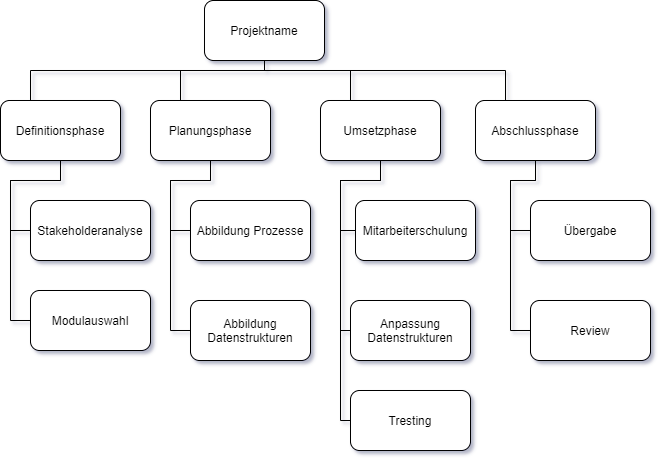
\includegraphics[width=15cm]{img/psp01.png}
		\caption{\ac{PSP}}
		\label{img:PSP1}
	\end{figure}
	
	
	
	
	
	\chapter{Handlungsempfehlung}
\label{chap:handlungs}

	Wie in der Einleitung bereits angedeutet beschäftigt sich die gicom AG mit der Implementierung von Standardsoftware, sowie deren Customizing. Da es sich bei dem von der gicom vertriebenen Produkt um ein im gewissen Rahmen erweiterbares Produkt handelt, kann es zu unterschieden in den Aufgabenstellungen kommen. Jedoch sind diese Abweichungen überschaubar. Bei der Implementierung buchen die meisten Kunden alle Module, da diese sich ergänzen. Nur wer alle Module besitzt kann das volle Potential der Software ausschöpfen. 
	Aus dem oben genannten Gründen kann das Customizing auch in drei Teile unterteilt werden. 
	
	\begin{itemize}
		\item Customizing \ac{AD}
		\item Customizing \ac{RTM}
		\item Customizing \ac{ANW}
	\end{itemize}

	Jedes dieser Tools sollte über einen eigenen \acs{PSP} verfügen. Diese klare Abgrenzung hilft der gicom nicht nur eine erhöhte Übersichtlichkeit zu bewahren, sondern verschafft auch Klarheit in Bezug auf die Zugehörigkeit der Aufgaben. Da das Modul der \ac{AD} die Voraussetzung schafft für die anderen Module sollte dies zuerst angegangen werden. Genau wie es im \autoref{chap:umsetzung} beschrieben wurde sollte hier ein phasenorientierter Ansatz verfolgt werden. Daher auch die unterschiedlichen Phasen als Grundlage für die weitere Aufgabenfindung gelten. Die Findung der unterschiedlichen \ac{AP} ist ein weiterer wichtiger Bestandteil des Prozesses. Neben den zur Verfügung gestellten Grundpfeilern des Customizings verfügt die gicom über ein immenses Set an Erfahrung und Aufgaben im Intranet, die aus vergangenen Projekten gesammelt wurden. Die Erläuterung beziehungsweise die Erstellung eines \acs{PSP} auf dieser Grundlage würde den Rahmen der Arbeit überschreiten. Indem der Autor eine Vorgehensweise für die korrekte Definition der \acs{AP} zur Verfügung gestellt hat, soll sichergestellt werden, dass nichts in bei der Erhebung vergessen wird. 
	Die \acs{PSP} der Tools \acs{RTM}, sowie \acs{ANW} sollten nach dem gleichen Verfahren erstellt werden. 
	
	\chapter{Fazit}

	Ziel dieser Arbeit war es herauszufinden, wie ein Projekt aufgebaut ist um darauf basierend ein generisches Konzept zu erstellen, welches für das Customizing eingesetzt werden kann. 
	
	Dazu wurden im \autoref{chap:projektablauf} die Zusammensetzung eines Projektes beschrieben. Hierbei wurde unter anderem auf die einzelnen Phasen eingegangen, auch der \ac{PSP} sowie das \ac{AP} wurden erläutert. Das \autoref{chap:SpecCustom}  hat die Themenbereiche des Customizings beleuchtet. Basierend auf diesen beiden Kapiteln konnten dann Erkenntnisse für die Umsetzung einer Strategie im \autoref{chap:umsetzung} gezogen werden. Das entwickelte Modell konnte dann im \autoref{chap:handlungs} in den Kontext der gicom gebracht werden.  
	
	Abschließend lässt sich festhalten, dass das Ziel dieser Arbeit, ein generisches Modell zu erstellen, teilweise erfüllt werden konnte. Es konnte ein Grundgerüst eines \ac{PSP} für das Customizing erstellt werden, jedoch hat der Rahmen dieser Arbeit es nicht zugelassen, sich tiefer mit den detaillierten Aufgabenstellungen des Customizings zu beschäftigen. Daher konnte auch kein Detaillierterer \acs{PSP} erstellt werden.  
	
	
	\printbibliography
\end{document}